%--------------------------------------------------------------
% thesis.tex 
%--------------------------------------------------------------
% Corso di Laurea in Informatica 
% http://if.dsi.unifi.it/
% @Facolt\`a di Scienze Matematiche, Fisiche e Naturali
% @Universit\`a degli Studi di Firenze
%--------------------------------------------------------------
% - template for the main file of Informatica@Unifi Thesis 
% - based on Classic Thesis Style Copyright (C) 2008 
%   Andr\'e Miede http://www.miede.de   
%--------------------------------------------------------------
\documentclass[twoside,openright,titlepage,fleqn,
	headinclude,11pt,a4paper,BCOR5mm,footinclude,pdftex
	]{scrbook}
%--------------------------------------------------------------
\usepackage{listings}
\usepackage{graphicx}
\newcommand{\myTitle}{Diametro in grafi orientati: calcolo di un limite inferiore\xspace}
% use the right myDegree option
\newcommand{\myDegree}{Corso di Laurea in Informatica\xspace}
%\newcommand{\myDegree}{
	%Corso di Laurea Specialistica in Scienze e Tecnologie 
	%dell'Informazione\xspace}
\newcommand{\myName}{Valerio Del Meglio\xspace}
\newcommand{\myProf}{Pierluigi Crescenzi\xspace}
\newcommand{\myOtherProf}{Nome Cognome\xspace}
\newcommand{\mySupervisor}{Nome Cognome\xspace}
\newcommand{\myFaculty}{
	Facolt\`a di Scienze Matematiche, Fisiche e Naturali\xspace}
\newcommand{\myDepartment}{
	Dipartimento di Sistemi e Informatica\xspace}
\newcommand{\myUni}{\protect{
	Universit\`a degli Studi di Firenze}\xspace}
\newcommand{\myLocation}{Firenze\xspace}
\newcommand{\myTime}{Anno Accademico 2010-2011\xspace}
\newcommand{\myVersion}{Version 0.1\xspace}
%--------------------------------------------------------------
\usepackage[utf8]{inputenc}
\usepackage{listings}
\lstloadlanguages{java}
%--------------------------------------------------------------
\usepackage{dia-classicthesis-ldpkg} 
%--------------------------------------------------------------
% Options for classicthesis.sty:
% tocaligned eulerchapternumbers drafting linedheaders 
% listsseparated subfig nochapters beramono eulermath parts 
% minionpro pdfspacing
\usepackage[eulerchapternumbers,subfig,beramono,eulermath,
	parts]{classicthesis}
%--------------------------------------------------------------
\newlength{\abcd} % for ab..z string length calculation
% how all the floats will be aligned
\newcommand{\myfloatalign}{\centering} 
\setlength{\extrarowheight}{3pt} % increase table row height
\captionsetup{format=hang,font=small}
%--------------------------------------------------------------
% Layout setting
%--------------------------------------------------------------
\usepackage{geometry}
\geometry{
	a4paper,
	ignoremp,
	bindingoffset = 1cm, 
	textwidth     = 13.5cm,
	textheight    = 21.5cm,
	lmargin       = 3.5cm, % left margin
	tmargin       = 4cm    % top margin 
}
%--------------------------------------------------------------
\begin{document}
\frenchspacing
\raggedbottom
\pagenumbering{roman}
\pagestyle{plain}
%--------------------------------------------------------------
% Frontmatter
%--------------------------------------------------------------
%--------------------------------------------------------------
% titlepage.tex (use thesis.tex as main file)
%--------------------------------------------------------------
\begin{titlepage}
	\begin{center}
   	\large
      \hfill
      \vfill
      \begingroup
			\spacedallcaps{\myUni} \\ 
			\myFaculty \\
			\myDegree \\ 
			\vspace{0.5cm}
         
\includegraphics[scale=.065]{logo/unifi}\\
         \vspace{0.5cm}    
         Tesi di Laurea    
      \endgroup 
      \vfill 
      \begingroup
      	\color{Maroon}\spacedallcaps{\myTitle} \\ \bigskip
      \endgroup
      \spacedlowsmallcaps{\myName}
      \vfill  
      Relatore: \itshape{\myProf}
      \vfill                   
      \myTime
      \vfill                      
	\end{center}        
\end{titlepage}   
%--------------------------------------------------------------
% back titlepage
%--------------------------------------------------------------
   \newpage
	\thispagestyle{empty}
	\hfill
	\vfill
	\noindent\myName: 
	\textit{\myTitle,} 
	\myDegree, \textcopyright\ \myTime
%--------------------------------------------------------------
% back titlepage end
%--------------------------------------------------------------
\pagestyle{scrheadings}
%--------------------------------------------------------------
% Mainmatter
%--------------------------------------------------------------
\pagenumbering{arabic}
% use \cleardoublepage here to avoid problems with pdfbookmark
%\include{intro} % use \myChapter command instead of \chapter
%\cleardoublepage\myPart{Part I}
%\include{chapter01}
%\cleardoublepage\myPart{Part II}
%\include{chapter02}
%\include{chapter03}
%\include{esercizi}



\chapter{Il diametro}
\section{Introduzione}
Nel contesto della teoria delle reti, un grafo complesso è un grafo con caratteristiche topologiche non banali, caratteristiche che non occorrono in semplici network come i grafi casuali ma che occorrono nei grafi reali.\\
Lo studio delle reti complesse è una giovane ed attiva area della ricerca scientifica ispirata largamente da studi empirici su reti del mondo reale come le reti di calcolatori o le reti sociali.\\Lo studio che qui si espone è focalizzato principalmente allla seconda tipologia, le reti sociali, intese come strutture composte da individui, organizzazioni o altre entità, inserite in un contesto sociale, che collaborano tra loro tramite delle relazioni ben definite.\\
\begin{center}
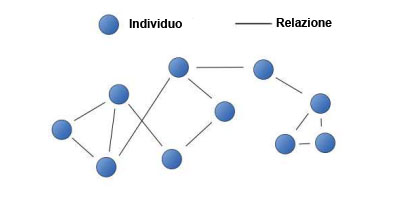
\includegraphics[width=13cm]{reti_sociali.jpg}
\caption{Figura: Reti sociali}
\end{center}

La maggior parte delle reti sociali mostra sostanziali caratteristiche topologiche non banali con schemi di connessione tra i propri elementi che non sono né puramente regolari né puramente casuali. Una di queste caratteristiche, nota come coefficiente di clustering, ci mostra ad esempio come in molte reti se il vertice A è connesso al vertice B e questo è connesso con il vertice C, allora con una buonà probabilità c'è una connessione anche tra il vertice A e il vertice C. Il riscontro di questa proprietà si può ritrovare nel fatto che spesso un amico di un nostro amico è anche nostro amico.\\
Uno dei più famosi studi condotti sulle reti, tanto da portarne alla divulgazione anche fuori dall'ambito scientifico, è quello noto  con il nome di "\textit{sei gradi di separazione}".\\Riprendendo dopo trent'anni gli scritti di un poeta ungherese di nome Frigyes Karinthy, che ipotizzava la possibilità di unire due persone sconosciute con un massimo di cinque passaggi intermedi, Stanley Milgram, un sociologo di Harvard, partì da quell'intuizione dando vita ad un originale ed avanzato studio sulla connettività delle persone.\\L'obiettivo di Milgram consisteva nel comprendere quale fosse la distanza che intercorreva tra due cittadini qualsiasi degli Stati Uniti. Come prima cosa il sociologo scelse due destinatari finali e inviò circa centosessanta lettere ad altri abitanti scelti casualmente. In ogni busta erano riportate delle brevi indicazioni sugli obiettivi dell'esperimento, una fotografia con il nome e l'indirizzo e poche altre informazioni sul destinatario finale e le istruzioni che la persona in questione avrebbe dovuto seguire per far pervenire la lettera alle due persone scelte. Grazie alle quarantadue delle centosessanta lettere che tornarono indietro, Milgram fu in grado di determinare che per raggiungere il destinatario finale fossero necessari in media 5,5 passaggi e da qui il concetto dei sei gradi di separazione.\\
Notiamo come, pur essendo stato un esperimento fondamentale per la comunità scientifica, quello di Milgram ci fornisce solo un'informazione sulla media delle distanze dei nodi all'interno di una rete e non sulla distanza massima tra una coppia di nodi. Tuttavia se il diametro di una rete cresce molto lentamente rispetto alla crescita della rete stessa, ad esempio \textit{O(log n)}, questa può essere definita di tipologia "piccolo mondo", rifacendosi agli esperimenti di Milgram.\\
Duncan Watts e Steve Strogatz, in un articolo scientifico del 1998 studiarono questo fenomeno usando un semplice modello matematico, ora chiamato "modello piccolo mondo". In questo modello, i vertici sono arrangiati circolarmente e connessi ai \textit{k} propri vicini. Poi con probabilità \textit{p} ogni vertice è connesso ad un altro nodo a formare una coppia di vertici. Quindi con \textit{p}=0 si ha una distribuzione degli archi completamente ordinata dove il coefficiente di clustering è maggiore e il diametro è \textit{O(n)},mentre con \textit{p}=1 la rete è completamente disordinata, il coefficiente di clustering è prossimo allo zero e il diametro è \textit{O(log n)}.\\
\begin{center}
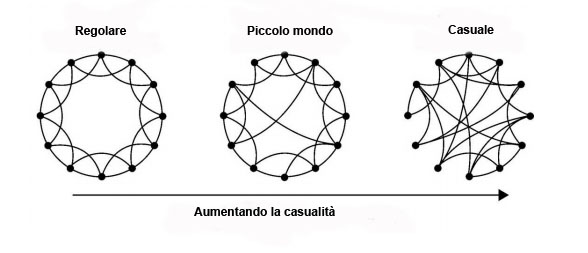
\includegraphics[width=14cm]{small_world.jpg}
\caption{Figura: Schema di Watts e Strogatz che illustra il modello piccolo mondo}
\end{center}
Watts e Strogatz scoprirono che il diametro di una rete variava da \textit{O(n)}, un "grande mondo" dove il più lungo cammino tra due nodi attraversava quasi l'intera rete, a \textit{O(log n)},un "piccolo mondo" dove la più lunga distanza tra due nodi attraversa una piccola parte della rete. Questo comportamento ricordava loro alcune proprietà delle reti sociali che hanno un piccolo diametro ma un'alta densità di triangoli, proprietà che molti modelli casuali non presentano simultaneamente.\\
Il risultato del piccolo mondo è interessante per molti motivi. Prima di tutto, esemplifica usando un modello, come le reti empiriche possano essere diverse dal semplice modello dei grafi casuali. Secondariamente mostra come certe misure sulla struttura di una rete possono essere estremamente sensibili rispetto alla struttura della stessa.

In questo contesto trova largo impiego lo studio del diametro di una rete complessa, ossia la massima tra le distanze tra ogni coppia di nodi, dove per distanza si intende il cammino minimo tra essi.\\
Il diametro di un grafo è uno dei parametri più importanti  per quanto concerne la teoria dei grafi e sta inoltre trovando sempre più sviluppi nell'analisi di reti complesse.
La sua importanza, come misura di studio, è dovuta alle osservazioni che tale parametro permette di compiere sulla forma o sulla struttura di un grafo, sull'idea di "grandezza" che ci può dare di una rete e per il design di algoritmi ad hoc su di una particolare rete.\\Si pensi ad esempio all'Internet Movie Database, conosciuto con il suo acronimo IMDb, questa è la più grande banca dati contenente informazioni relative a film, attori, registi e tutto quanto ciò che riguarda il cinema; Proprio grazie alle interfacce a riga di comando che lo stesso IMDb mette a disposizione, è possibile estrapolare le informazioni che ci servono per poi trattarle come reti per i nostri scopi. In particolare se i nodi della nostra rete sociale rappresentano gli attori e gli archi collegano due attori che hanno collaborato in almeno un film, calcolare il diametro di questo tipo di grafi di anno in anno, dove in ognuno le relazioni tra attori sono intese solo sull'anno in esame, ci può dare una stima di quanto cresca il mercato del cinema o di quanti attori diversi siano stati impiegati.\\
Questo ci consente, inoltre, di porre un upper bound sulla lunghezza delle connessioni che stiamo studiando. Molti ricercatori infatti limitano le proprie esplorazioni sulla connessioni includendo solo connessioni che non eccedano il valore del diametro della rete.\\
Altri studi di sono concentrati sulla crescita o sulla decrescita del diametro in base a vari fattori, ad esempio studi dell'università di Stanford hanno mostrato come, contrariamente a quanto si possa pensare, il diametro di vari datasets sperimentati decresca con il tempo nonostante aumenti il numero totale dei nodi.\\Altre congetture si sono fatte su reti sociali in cui i nodi sono di tipologia diverse; Dato quindi un insieme di nodi partizionati in gruppi dove i nodi facenti parte di uno stesso gruppo sono della stessa tipologia, ci si chiede come, tenendo costante la distribuzione dei gradi, si possa evolvere una rete di nodi di questo tipo comparata ad una rete in cui queste differenze sono ignorate. Credenza comune potrebbe essere quella di pensare che, aumentando l'omofilia, aumenti anche la probabilità di collegamenti tra nodi dello stesso tipo e decresca la probabilità di collegamenti tra nodi di tipologie differenti.Tuttavia questi studi hanno mostrato come anche quando decresce la probabilità di collegamenti tra tipologie, la distanza media e il diametro non cambiano mentre grosso impatto si ha sul coefficiente di clustering, dove un sostanziale livello di omofilia porta ad un clustering non banale, contrariamente a quanto avviene su di una rete priva di omofilia.

Tuttavia gli algoritmi noti per il suo calcolo, anche quelli che producono valori approssimativi, sono eccessivamente esosi in termini di spazio e/o tempo.\\
L'approccio che qui si propone per il calcolo del diametro è un semplice e veloce metodo per determinare un lower bound per il diametro di grafi orientati che, spesso e volentieri, coincide con il diametro stesso o che comunque, si discosta di poco da esso.\\
\\
In questo elaborato, si considera un grafo diretto, non pesato,\textit{G=(V,E)} con \textit{n=$\mid $V$\mid $} vertici  e \textit{m=$\mid$E$\mid$} archi.
Si denota con \textit{d(u,v)} la distanza tra il vertice \textit{u} e il vertice \textit{v}, con \textit{ecc(v)} l'eccentricità del vertice \textit{v}, ossia la massima distanza tra il vertice \textit{v} e ogni altro vertice \textit{u} del grafo e infine con \textit{D}=$max_u_,_v  $\textit{d(u,v)}=$max_v$ \textit{ecc(v)},il diametro di \textit{G}.\\
Calcolare tutte le distanze da un vertice verso tutti gli altri (e così la sua eccentricità) ha un costo di tempo e spazio pari a \textit{O(m)} usando una visita in ampiezza (BFS). Per ottenere dunque il diametro, questa eccentricità deve essere calcolata per ogni vertice del grafo per un costo temporale complessivo pari a \textit{O(n$\cdot $m)} usando \textit{n} BFS.\\Anche usando l'algoritmo di Dijkstra per calcolare il cammino minimo da un vertice verso tutti gli altri si ottiene una complessità proibitiva su grafi più complessi, in quanto l'algoritmo deve essere eseguito su ogni nodo del grafo per ottenere tra questi cammini il valore massimo che corrisponde al diametro.\\

\section{Lavori correlati}
Diventando una fondamentale proprietà dei grafi, la determinazione del diametro, è lo scopo principale di numerose ricerche in ambito informatico. Gli algoritmi per il calcolo del diametro, solitamente appartengono alle seguenti categorie.
\begin{itemize}

\item Moltiplicazioni tra matrici.\\
Questi algoritmi, che permettono inoltre di risolvere il problema \textit{All-Pairs Shortest Path} del calcolo del cammino minimo da un vertice \textit{u} verso ogni altro vertice \textit{v}, sostanzialmente iterano la moltiplicazione delle matrici delle distanze del grafo e generalmente si applicano a tutti i tipi di grafi (diretti o non diretti,pesati o non pesati).\\L'idea generale è quella di mantenere per ogni coppia di vertici (\textit{u,v}) un valore che tenga memoria del fatto che non sono conosciuti cammini minimi oltre a quello segnalato; Proseguendo nella navigazione del grafo i valori corrispondenti ai cammini minimi tra due vertici vengono aggiornati qualora si trovi un cammino più breve. Il più grande elemento della matrice rappresenterà il diametro.\\
D'altro canto sorgono dei problemi di memoria quando si cerca di applicare questa tipologia di algoritmi su grafi di grandezza maggiore, in quanto è necessaria la memorizzazione di una matrice \textit{N}x\textit{N}.\\Difatti il metodo migliore facente parte a questa categoria permette di eseguire le operazioni con un tempo di calcolo asintoticamente pari a \textit{O}(\textit{N^3$}).



\item Algoritmi che lavorano su certe tipologie di grafi.\\
Date delle specifiche condizioni sulla distribuzione dei gradi dei vertici, possono essere trovati dei Lower e Upper bounds che però, generalmente non corrispondono all'esatto valore del diametro.
Tuttavia alcune stime sui bounds si sono poi rilevate corrette ad esempio nei grafi cordali, ossia grafi in cui ogni ciclo di lunghezza maggiore o uguale a quattro ha una corda, cioè un arco tra due nodi non adiacenti nel ciclo.
\begin{center}
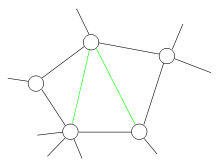
\includegraphics[width=08cm]{cordale.png}\\
\caption{Figura: grafo cordale}
\end{center}

\item Approssimazioni o testing del diametro.\\
Alcuni algoritmi eseguono una campionatura costante dell'eccentricità del grafo, eseguendo un numero fissato di BFS, come ad esempio è indicato sulla homepage dello Stanford Network Analysis Platform (successivamente indicato con SNAP) o calcolano un'approssimazione solamente su di un campione dei nodi del grafo. Prendendo dunque un largo ma gestibile campione di nodi è possibile calcolare per ciascuno le distanze verso gli altri e prendere la maggiore come approssimazione del diametro. Ovviamente questo approccio è dipendente dalla campionatura iniziale che si effettua e dalla struttura del grafo ,quindi non si hanno bounds utili in caso di sbagliate campionature né tantomeno un'approssimazione certa del diametro.

\end{itemize}
\chapter{Strumenti algoritmici}
In questo capitolo si mostrano gli strumenti che hanno permesso la realizzazione dell'algoritmo.
L'algoritmo che esegue la visita in ampiezza, utilizza un array booleano, in cui il valore \textit{true} è attribuito ad un nodo già visitato nel corso della visita al fine di esaminare ogni arco un numero non infinito di volte. Dopo aver inizializzato l'array booleano e l'array delle distanze, viene iniziata la visita inserendo in coda l'id del nodo su cui è stato invocato il metodo; Inizialmente l'unico nodo presente in coda verrà estratto e così inseriti in coda i suoi figli se non esaminati precedentemente. Grazie all'array booleano, ciascun nodo, e così le sue liste di adiacenza, verrà visitato una volta sola, ottenendo un costo totale della visita pari alla somma delle lunghezze delle liste di adiacenza esaminate.\\
Ad arricchire l'algoritmo è stato utilizzato un ulteriore array \textit{dist} che restituisce le distanze dei vari nodi dal nodo di partenza della visita in modo da estrapolare da esso l'indice del nodo a distanza massima tramite il metodo \textit{GetIndexOfMax}.\\

\lstinputlisting[language=Java]{BFS.java}
\\
\lstinputlisting[language=Java]{Getindexofmax.java}
\newpage
Utilizzando invece una visita in profondità ricorsiva, è stato possibile implementare l'algoritmo per trovare la componente fortemente connessa più grande.\\Inizialmente nessun nodo è visitato e le pile sono vuote, l'array \textit{dfsnumber} viene usato sia per numerare i nodi in ordine di scoperta (attraverso \textit{counter} ) sia per verificare se un nodo è già stato visitato o meno. Partendo da un nodo del grafo, lo si inserisce nelle pile per poi esaminare i vertici adiacenti al nodo precedentemente inserito e invocare ricorsivamente la visita sui vertici non ancora raggiunti. A differenza delle semplici visite in ampiezza e in profondità, anche se un nodo è già stato visitato, occorrerà verificare se l'arco tra esso e il nodo di partenza forma un ciclo,possibile solo se il nodo in esame non è completo, ossia se la visita di tutti i suoi vertici adiacenti non è stata completata. In tal caso si ha un ciclo di componenti parziali ed occorrerà rimuovere dalla pila dei parziali i rappresentanti di tali componenti. L'unico nodo che rimane, quello con numerazione di visita minore,diviene il rappresentante della nuova componente parziale così creata e, terminata la scansione del vertice di partenza,abbiamo che esso diventa completo poiché non è più possibile scoprire ulteriori vertici da quest'ultimo. Se il nodo è anche rappresentante della propria componente, significa che forma una nuova componente completa insieme ai vertici che si trovano sopra di esso nella pila dei parziali e sarà quindi necessario estrarre ciascuno di questi vertici dalla pila \textit{partial}, marcarli come completi ed eliminare il nodo di partenza dalla pila dei rappresentanti.
Dati i nodi che occorrono più frequentemente ci è così possibile restituire la componente fortemente connessa più grande.\newpage
Codice del metodo che implementa la ricerca della componente fortemente connessa più grande.
\lstinputlisting[language=Java]{SCC.java} \newpage
\lstinputlisting[language=Java]{SCC2.java}

\newpage
Si mostra adesso un  esempio di esecuzione dei due metodi sul semplice grafo presente in figura.
\begin{center}
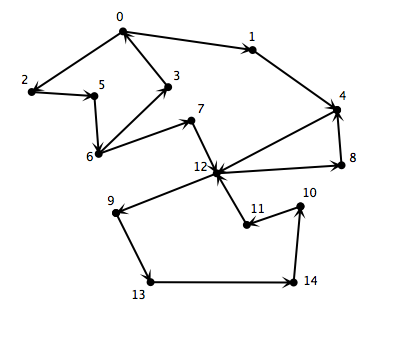
\includegraphics[width=10cm]{grafoesempio2}
\end{center}
Per prima cosa si esegue l'algoritmo per il calcolo della componente fortemente connessa più grande. Questo ci restituirà la componente fortemente connessa formata dai nodi 4, 8, 9, 10, 11, 12, 13, 14. Successivamente gli indici di questi nodi vengono rimappati e stampati su un file di testo in modo da considerare questo sottografo come un grafo a sé stante.
\begin{center}
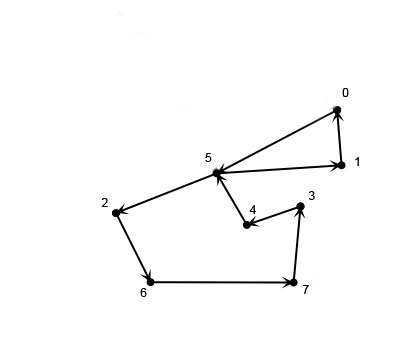
\includegraphics[width=10cm]{grafoesempio2cc.jpg}
\end{center}
A questo punto l'esecuzione del metodo \textit{BFS} ci restituisce le distanze dei nodi dato uno di partenza. Supponendo di eseguire la visita dal nodo di indice 0 (notiamo che avendo rimappato i nodi questo corrisponda al precedente indice 4) l'algoritmo ci restituirà il seguente array di distanze: [0 2 2 5 6 1 3 4] dove ovviamente il valore in posizione \textit{i} indica la distanza dal nodo di partenza al nodo i-esimo.
\chapter{Double sweep}
L'idea alla base dell'algoritmo che qui si presenta è quella di calcolare due valori, un lower bound $\underline{D}$ e un upper bound $\overline{D}$ tali che $\underline{D}$ $\leq$ D $\leq $ $\overline{D}$.
Il metodo è tanto semplice quanto efficace, in quanto consente di ottenere un lower bound che poco si discosta dal valore del diametro o che talvolta è equivalente. Notiamo come, eseguendo una BFS da un nodo del grafo, l'altezza dell'albero corrispondente sarà al più, grande quanto il diametro stesso ma non eccederà mai questo valore essendo la distanza dal nodo radice a uno dei nodi dell'ultimo livello dell'albero, il cammino minimo tra i due.\\Infatti, per ogni vertice v si ha che \textit{ecc(v)} $\leq$ D $\leq$ \textit{2}$\cdot $ \textit{ecc(v)}, per cui l'eccentricità di ogni vertice \textit{v} ci dà un trivial bound,ossia un'approssimazione sul lower o sull'upper bound che chiameremo appunto trivial lower e upper bounds e che può essere calcolata in \textit{O(m)} spazio e tempo. La qualità del trivial bound  dipende ovviamente dalla scelta del vertice \textit{v}.\\Per alcune specifiche classi di grafi, alberi inclusi, se \textit{v} è scelto in modo da avere\textit{ d(u,v)=ecc(u)} per un vertice \textit{u} allora \textit{D=ecc(v)}.\\Per queste classi di grafi il diametro può quindi esser calcolato con una BFS da un nodo \textit{u} e poi con una BFS da un nodo alla massima distanza da \textit{u}. Otteniamo così una migliore approssimazione del lower bound di quella ottenuta per il trivial bound dallo stesso vertice (che calcola \textit{ecc(u))}.\\


Dato dunque un grafo diretto, prima di tutto viene calcolata la componente connessa più grande, dato che è uso comune nella letteratura scientifica ricercare il diametro al suo interno e per escludere eventuali nodi non connessi (notiamo come se il grafo non fosse connesso il diametro sarebbe considerato infinito).\\Dopo il calcolo della componente connessa più grande, l'intero algoritmo si svolge con due semplici  visite in ampiezza, la prima, da un nodo scelto casualmente, la seconda da uno dei nodi posti alla distanza massima dal nodo precedentemente scelto, ma invertendo l'orientamento degli archi del grafo.\\Il lower bound scelto, è il valore massimo tra le due altezze degli alberi ottenuti dalle corrispettive visite in ampiezza. Si nota comunque come, nelle prove effettuate, il valore scelto sia sempre stato quello corrispondente all'esecuzione della seconda BFS, e come anzi il valore corrispondente alla prima BFS fosse prossimo alla metà del diametro reale.\\
Il vantaggio di questo approccio in ottica di tempo e spazio è enorme, si ha infatti quasi la garanzia di trovare il diametro reale dopo un numero arbitrariamente basso di esecuzioni iterando da diversi nodi casuali al costo di poche visite in ampiezza. Già su grafi con alcune decine di migliaia di nodi la differenza tra questo metodo e il metodo esaustivo è sostanziale.\\


\section{Implementazione}\\
L'algoritmo è stato implementato usando Java, i grafi sono stati rappresentati come liste di adiacenza, una per l'orientamento originale del grafo e una con l'orientamento degli archi invertito da utilizzare per effettuare la seconda BFS.\\Queste ultime sono state realizzate tramite array bidimensionali e non tramite array dinamici per un miglior utilizzo della memoria in quanto i primi consentono di ottenere informazioni quali la lunghezza dell'array o l'elemento all'i-esimo posto in tempo costante, mentre le seconde iterano sull'intera lista rendendo l'intero algoritmo decisamente meno efficiente quando si trattano dati più consistenti.
Sempre nell' ottica di ottimizzare la memoria, i grafi sono letti da file di testo composti, rispettivamente, da: numero totale dei nodi, in degree e out degree che indicano per ogni nodo il numero di archi incidenti e il numero di archi uscenti, lista degli archi indicati come coppie di nodi in cui il secondo è il nodo su cui l'arco è incidente.\\Pertanto sono state implementate delle opportune classi parser  per convertire i dataset utilizzati come test in questo formato. Leggendo, dunque, il file composto in questo modo, sappiamo immediatamente, dato il numero totale dei nodi, quanta memoria allocare per il primo array e,successivamente, dati i degree dei nodi, quanta memoria allocare per gli array contenuti nel primo;\\
Leggendo infine gli archi, l'algoritmo semplicemente popola gli array corrispondenti all'id del nodo che ha letto. L'unico limite hardware è, ovviamente, che il numero dei dati non superi la quantità di memoria centrale altrimenti sarebbe necessario eseguire degli swap di memoria che ne degraderebbero le prestazioni.
Come detto in precedenza, prima di tutto è necessario calcolare la componente connessa più grande e lavorare su di essa; per cui una volta letto il file del grafo nel formato corretto e popolate le liste di adiacenza, viene calcolata la componente connessa più grande e a sua volta viene stampata su un file effettuando un opportuno remapping dei vertici; Una prima BFS a partire da un nodo casuale del grafo restituisce un primo lower bound, non molto accurato mentre una seconda BFS a partire da uno dei nodi all'ultimo livello dell'albero ottenuto con la BFS precedente restituisce il secondo lower bound, che nelle prove effettuate è sempre quello scelto in quanto più accurato.\\
Di seguito l'algoritmo java utilizzato, dove \textit{BFS} è il metodo che implementa la visita in ampiezza, \textit{getIndexOfMax} restituisce l'indice dell'ultimo nodo all'ultimo livello dell'albero ottenuto con la \textit{BFS}, infine \textit{graphfw} rappresenta il grafo con l'orientamento degli archi originale e \textit{graphbw} lo stesso grafo ma con l'orientamento degli archi invertito.\\\\ \newpage
\caption{Algoritmo Java}
\lstinputlisting[language=Java]{algoritmo.java}

\\
\\
\section{Esempio di esecuzione}\\
Di seguito un esempio su un semplice grafo in cui si mostra l'esecuzione dell'algoritmo da due nodi di partenza differenti.
\begin{center}
\includegraphics[width=10cm]{/users/valerio/Desktop/grafotesirit}
\end{center}
Supponiamo di scegliere come nodo di partenza il nodo con indice 8 ed eseguire la prima BFS a partire da esso.
Si ottiene il seguente albero in cui il nodo di indice 4 è stato escluso in quanto non facente parte della componente fortemente connessa.
\begin{center}
\includegraphics[width=10cm]{/users/valerio/Desktop/albero1rit}
\end{center}
Come da algoritmo, invertiamo l'orientamento degli archi del grafo ed eseguiamo un'altra BFS a partire da uno dei nodi all'ultimo livello dell'albero, in questo caso il nodo di indice 9.
I risultati ottenuti sono mostrati nelle seguenti due figure:
\begin{center}
\includegraphics[width=10cm]{/users/valerio/Desktop/grafotesirev}
\end{center}
\begin{center}
\includegraphics[height=8cm]{/users/valerio/Desktop/albero2rev}
\end{center}
L'altezza dell'albero così ottenuto, mostrato nell'ultima figura, corrisponde così al diametro del grafo di partenza, come facilmente verificabile, date le dimensioni del grafo in questione, eseguendo l'algoritmo dei cammini minimi da ogni nodo.\\
Viene mostrata adesso l'esecuzione dell'algoritmo a partire da un altro nodo, sia esso il nodo di indice 0.
Di seguito i due alberi ottenuti dalle rispettive due BFS.
\begin{center}
\includegraphics[width=10cm]{/users/valerio/Desktop/alberidue}
\end{center}
L'altezza del secondo albero, non coincide in questo modo con il diametro corretto, essendo la prima 4 mentre il secondo 8.\\Tuttavia su un grafo campione come questo, su dieci nodi, l'algoritmo sbaglia a calcolare il diametro solamente partendo dal nodo di indice 0, mentre lo calcola correttamente partendo da tutti gli altri.\newpage
Si mostra inoltre come tuttavia non sia difficile progettare una rete in cui il comportamento dell'algoritmo non sia ottimale. Facciamo riferimento alla figura che segue:
\begin{center}
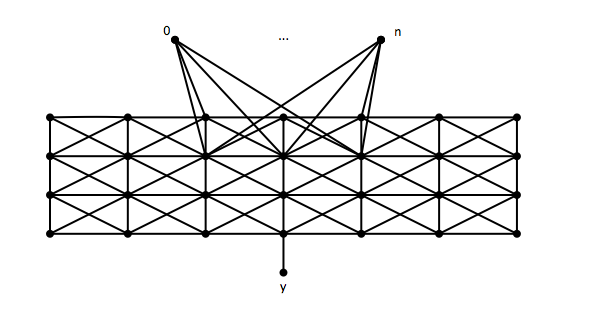
\includegraphics[width=12cm]{cattivoesempio}
\end{center}
Si consideri appunto una griglia con \textit{k} righe e 1+3\textit{k}/2 colonne. Ogni vertice della griglia è connesso agli altri vertici con una distanza di al più \sqrt{2}$ ma ci sono \textit{n} vertici addizionali \textit{$x_0$}...\textit{$x_n$} che sono connessi ai vicini del vertice in mezzo alla prima riga e un ulteriore vertice \textit{y} che è connesso con il vertice in mezzo all'ultima riga. Si può notare come, per \textit{n} sufficientemente grande rispetto a \textit{k} l'algoritmo rischi di eseguire una prima \textit{BFS} fino al vertice \textit{y} per poi eseguirne una seconda a partire da \textit{y}. La seconda \textit{BFS} avrà altezza pari a \textit{k}+1 mentre è facile mostrare come il diametro della rete sia 3\textit{k}/2.
Nonostante il grafo scelto sia non orientato, possiamo comunque interpretarlo come un grafo in cui ogni arco ha una doppia orientazione e il risultato di quanto visto sopra non varierà.
\\
\\
\chapter{Esperimenti}
\section{Datasets}Sono stati raccolti circa 50 grafi cercando di ricoprire varie tipologie di network, dalle reti stradali alle reti sociali. Di seguito l'elenco dei grafi utilizzati, catalogati in base alla provenienza.
\begin{enumerate}
\item Snap (http://snap.stanford.edu/data/index.html)
\begin{itemize}
\item Network internet peer-to-peer:\\
\textit{p2p-gnutella04,p2p-gnutella06,p2p-gnutella08,p2p-gnutella09,p2p-gnutella24,p2p-gnutella25,p2p-gnutella30,p2p-gnutella31}
\item Grafi web:\\
\textit{ web-Notredame,web-Stanford  }
\item Network di comunicazioni e network sociali:\\
\textit{email-Enro,email-EuAll,soc-Epinions1,soc-Slashdot0811,soc-Slashdot0902}
\end{itemize}
\item Dimacs (http://www.dis.uniroma1.it/~challenge9/download.shtml)
\begin{itemize}
\item Reti stradali:\\
\textit{Colorado,New York,San Francisco Bay Area}
\end{itemize}
\item Boards and Gender (http://www.boardsandgender.com/data.php)
\begin{itemize}
\item Grafi sulla rappresentanza dei sessi in Norvegia:\\
\textit{net1m_2002-05-01,net1m_2002-07-01,net1m_2002-09-01,net1m_2002-11-01,net1m_2003-01-01,net1m_2003-03-01,net1m_2003-05-01,net1m_2003-07-01,net1m_2003-09-01,net1m_2003-11-01,net1m_2004-01-01,net1m_2004-03-01,net1m_2004-05-01,net1m_2010-11-01,net1m_2011-03-01,net1m_2011-05-01,net1m_2011-07-01}$
\end{itemize}
\item Tore Opsahl (http://toreopsahl.com/datasets/)
\begin{itemize}
\item Rete neurale del verme Caenorhabditis elegans:\\
\textit{C.elegans Neural Network}
\item Partecipazioni sociali\\
\textit{Davis’ Southern Women Club}
\item Social Network e Forum Network\\
\textit{Facebook-like Social Network,Facebook-like Forum Network}
\item Network di Freeman\\
\textit{Freeman’s EIES dataset(personal relationships;time 1),Freeman’s EIES dataset(personal relationships;time 2),Freeman’s EIES dataset(messages)}
\item Network di collaborazione Scientifica di Newman\\
\textit{Newman’s scientific collaboration network}
\item Network di tre aereoporti statunitensi\\
\textit{USairport500,USairport\textunderscore 2010Openflights}
\item Grafo di una rete elettrica statunitense\\
\textit{USpowergrid\textunderscore n4941}\\
\end{itemize}
\item Pajek (http://vlado.fmf.uni-lj.si/pub/networks/data/)
\begin{itemize}
\item Interazioni tra proteine nel lievito\\
\textit{Yeast}
\item Set di associazioni di parole \\
\textit{EAT response-stimulus}
\end {itemize}
\item Uci (http://www-personal.umich.edu/~mejn/netdata/)
\begin{itemize}
\item Network neurale\\
\textit{Celegansneural}\\
\end{itemize}
\end{enumerate}


\section{Risultati ottenuti}

\begin{center}
\begin{tabular}{|r|c|c|c|}
\hline
Nome grafo&Diametro esatto&Lb dopo 1 esecuzione&lb  dopo 10 esecuzioni\\ \hline
email-Enron&13&13&13\\ \hline
email-Euall&10&9&10\\ \hline
p2p-gnutella04&25&21&25\\ \hline
p2p-gnutella06&19&19&19\\ \hline
p2p-gnutella09&19&18&19\\ \hline
p2p-gnutella24&28&28&28\\ \hline
p2p-gnutella25&21&19&21\\ \hline
p2p-gnutella30&23&22&23\\ \hline
p2p-gnutella31&30&30&30\\ \hline
soc-Epinions1&16&16&16\\ \hline
soc-Slashdot0811&12&12&12\\ \hline
soc-Slashdot0902&13&12&13\\ \hline
web-NotreDame&93&93&93\\ \hline
web-Stanford&210&210&210\\ \hline
\end{tabular}
\end{center}





















%--------------------------------------------------------------
\end{document}
%--------------------------------------------------------------
